
\section{Struttura e Componenti del Sistema}

\subsection{Sistema di Bidding}

Il sistema di bidding permette ai manager della banca di definire una serie di regole di bidding che permettano ai clienti della banca di effettuare proposte (bid) verso un insieme di oggetti di bid messi a disposizione dalla banca.

L'insieme di oggetti di bid comprende:
\begin{itemize}
	\item conti correnti;
	\item carte di credito;
	\item prestiti.
\end{itemize}

Ciascuna regola prende in considerazione dei \emph{parametri di decisione} rispetto ai quali stabilire se accettare o rifiutare (o rimandare a un manager) dei \emph{parametri di bid} relativi all'oggetto in questione.

I parametri di decisione per ogni oggetto comprendono:
\begin{itemize}
	\item giacenza media su base mensile o annuale sui conti correnti del cliente;

	\item affidabilità del cliente misurata come percentuale di tempo in cui i conti correnti sono stati coperti;

	\item valore totale stipendi e/o pensioni accreditati sui conto corrente del cliente.
\end{itemize}

I parametri di bid per le carte di credito comprendono:
\begin{itemize}
	\item prelievo massimo giornaliero;

	\item prelievo massimo mensile;

	\item spese di commissione.
\end{itemize}

Per ogni oggetto di bid, il prodotto cartesiano dei domini dei parametri di decisione e dei parametri di bid dell'oggetto costituisce il \emph{dominio di bidding} dell'oggetto in questione.
Il bid di un cliente della banca per un certo oggetto identifica univocamente un elemento nel dominio di bidding dell'oggetto in questione.

Per ogni oggetto di bid, il sistema di regole di bid è implementato come un insieme di vincoli lineari sul dominio di bidding.
I vincoli lineari sono di due tipi:
\begin{itemize}
	\item vincoli di approvazione automatica;

	\item vincoli di approvazione supervisionata.
\end{itemize}

Un elemento del dominio di bidding che soddisfi tutti i vincoli di approvazione automatica è approvato automaticamente.

Un elemento del dominio di bidding che non soddisfi tutti i vincoli di approvazione automatica ma che soddisfi tutti i vincoli di approvazione supervisionata viene inviato ad un manager per l'eventuale approvazione.

Un elemento del dominio di bidding che non soddisfi tutti i vincoli di approvazione automatica e che non soddisfi tutti i vincoli di approvazione supervisionata viene rifiutato automaticamente.

\subsubsection{Visualizzazione dei Domini di Bidding}

Per ciascun oggetto di bid, il sottoinsieme del dominio di bidding costituito dagli elementi che soddisfino tutti i vincoli di approvazione automatica costituisce l'insieme dei bid approvati automaticamente.

L'unione dell'insieme dei bid approvati automaticamente e del sottoinsieme del dominio di bidding costituito dagli elementi che soddisfino tutti i vincoli di approvazione supervisionata costituisce l'insieme dei bid soggetti ad approvazione supevisionata.

L'insieme dei bid approvati automaticamente è un sottoinsieme (possibilmente improprio) dei bid soggetti ad approvazione supervisionata.

Per visualizzare gli insiemi di bid approvati automaticamente e di bid soggetti ad approvazione supervisionata i manager possono sfruttare due metodologie:
\begin{enumerate}
	\item visualizzare i \emph{punti estremi} degli insiemi di bid approvati automaticamente e dei bid soggetti ad approvazione supervisionata;

	\item ottenere una rappresentazione grafica dei due insiemi rispetto a due assi, ossia due parametri scelti fra l'unione dei parametri di decisione e dei parametri di bid, con i valori degli altri parametri fissati.
	Un esempio di questo tipo di rappresentazione grafica è indicato in figura~\ref{fig:visualization-bidding}.
	L'area verde indica l'insieme dei bid approvati automaticamente, mentre l'area arancio indica l'insieme dei bid soggetti ad approvazione supervisionata.
\end{enumerate}

\begin{figure}
\centering
	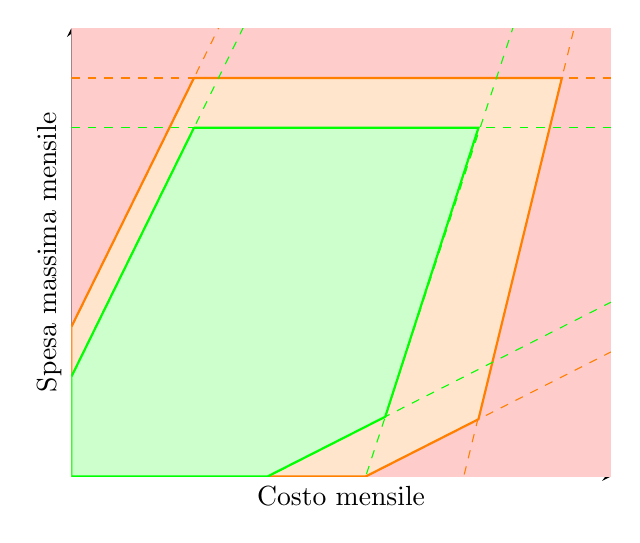
\begin{tikzpicture}
		\begin{axis}[
			ticks=none,
			domain=0:11,
			ylabel={Spesa massima mensile},
			xlabel={Costo mensile},
			axis y line = left,
			axis x line = bottom,
			samples     = 160,
			xmin = 0, xmax = 11,
			ymin = 0, ymax = 9,
		]
		    \addplot [draw=none, fill=red!20] coordinates {(0, 0) (12, 0) (12,12) (0,12)};
		    \addplot[name = b1, orange, dashed] {2 * x + 3};
		    \addplot[name = b2, orange, dashed] {1/2 * x - 3};
		    \addplot[name = b3, orange, dashed] {8};
		    \addplot[name = b4, orange, dashed] {4 * x - 32};
		    \addplot [orange, thick, fill=orange!20] coordinates
		    	{(2.5,8) (10,8) (8.3,1.15) (6,0) (0,0) (0,3) (2.5, 8)};
		    \addplot[name = a1, green, dashed] {2 * x + 2};
		    \addplot[name = a2, green, dashed] {1/2 * x - 2};
		    \addplot[name = a3, green, dashed] {7};
		    \addplot[name = a4, green, dashed] {3 * x - 18};
		    \addplot [green, thick, fill=green!20] coordinates
		    	{(2.5,7) (8.3,7) (6.4,1.2) (4,0) (0,0) (0,2) (2.5, 7)};
		\end{axis}
	\end{tikzpicture}
	\caption{Un esempio di visualizzazione di bidding: confronto fra spesa massima mensile di una carta di credito e costo di mantenimento della stessa.}
	\label{fig:visualization-bidding}
\end{figure}

\subsubsection{Considerazioni sul Sistema di Bidding}

Il sistema di bidding proposto ha i seguenti vantaggi:
\begin{itemize}
	\item le regole di bidding sono definite tramite disequazioni lineari, per le quali abbondano la teoria e i metodi di risoluzione;

	\item poiché le regole sono costituite da disequazioni lineari è facile analizzare il comportamento del sistema di bidding \emph{agli estremi}, ossia verificare i bid ``peggiori'' e ``migliori'' che il sistema approverebbe automaticamente;

	\item per il management della banca è possibile implementare regole non lineari di approvazione dei bid sfruttando l'insieme di bid soggetti ad approvazione supervisionata.
\end{itemize}

Gli svantaggi del sistema di bidding proposto sono i seguenti:
\begin{itemize}
	\item la visualizzazione di vincoli lineari su molte variabili può essere controintuitiva.
\end{itemize}

\subsection{Classi di Analisi}


Nei diagrammi seguenti sono illustrate alcune delle classi del sistema di HBS.
Per l'analisi e il design del sistema riteniamo sia di maggior rilievo uno studio approfondito dell'interazione fra i componenti dello stesso.

